\documentclass{article}
\usepackage{graphicx} % Required for inserting images

\usepackage[backend=biber]{biblatex}
\addbibresource{Bibliography.bib}


\title{The Fuzzy Logic Controller Used in the Moonrat~II}
\author{Horacio García--Vázquez}
\date{April 2026}

\begin{document}

\maketitle

\section{Fuzzy Logic Controller Strategy}

Precise and adaptive temperature control is essential in cultivation chambers for Petrifilm samples. To achieve this, we implemented a \textit{Mamdani--type fuzzy controller}. This approach is efficient and easy to apply to systems with slow dynamic evolution, such as temperature and heat control processes \cite{Sherif2014,Vijayalakshmi2017,Izquierdo2018,Coban2019,Sakaci2021}. 

To enable integration into an embedded system, we employed the \textit{Embedded Fuzzy Logic Library (eFLL)} developed by AJ Alves \cite{eFLL}. This library provides a standardized implementation of fuzzy control for embedded computing platforms.  

The system relies solely on measuring the chamber temperature and a predefined reference value. Consequently, we designed a \textit{Mamdani--based fuzzy control scheme} with two input variables:
\begin{itemize}
\item \textbf{Error} ($e$): The difference between the measured temperature $temp_c$ and the desired temperature $temp_r$:
\begin{equation}
e = temp_c - temp_r
\end{equation}

\item \textbf{Error difference} ($\Delta e$): The discrete change in error between two sampling instants:
\begin{equation}
\Delta e = e(t_k) - e(t_k - 1)
\end{equation}
\end{itemize}

We defined both input variables using three fuzzy sets: \textit{negative, zero, and positive}. We established the relationship between these variables and the controller’s response through a \textit{set of fuzzy rules}, as detailed in Table~\ref{tab:fuzzy_rules}.  

\begin{table}[h]
\centering
\renewcommand{\arraystretch}{1.3}
\setlength{\tabcolsep}{10pt}
\begin{tabular}{cc|ccc}
\hline\hline
\multicolumn{2}{c|}{\multirow{2}{*}{\textbf{Control}}} & \multicolumn{3}{c}{\textbf{Error Difference}} \\ 
\cline{3-5}
\multicolumn{2}{c|}{} & \textbf{Negative} & \textbf{Zero} & \textbf{Positive} \\ 
\hline\hline
\multirow{3}{*}{\textbf{Error}} 
& \textbf{Negative} & P & P & Z \\ \cline{2-5}
& \textbf{Zero}     & P & Z & N \\ \cline{2-5}
& \textbf{Positive} & Z & N & N \\ 
\hline\hline
\end{tabular}
\caption{Fuzzy control rule table. P = Positive, Z = Zero, N = Negative.}
\label{tab:fuzzy_rules}
\end{table}


The system's output variable is the \textit{PWM frequency}, which regulates the power supplied to the thermal pad responsible for heating the chamber. We defined this output using three fuzzy sets: \textit{high, medium, and low frequency}.  

We carried out the fuzzy system design, including the membership functions of the input and output variables, using the \textit{Fuzzy Logic Designer} toolbox in MATLAB.~Figure~\ref{fig:membership_functions} illustrates the configuration of the membership functions and the assigned ranges for each fuzzy set.

\begin{figure}[ht]
\centering
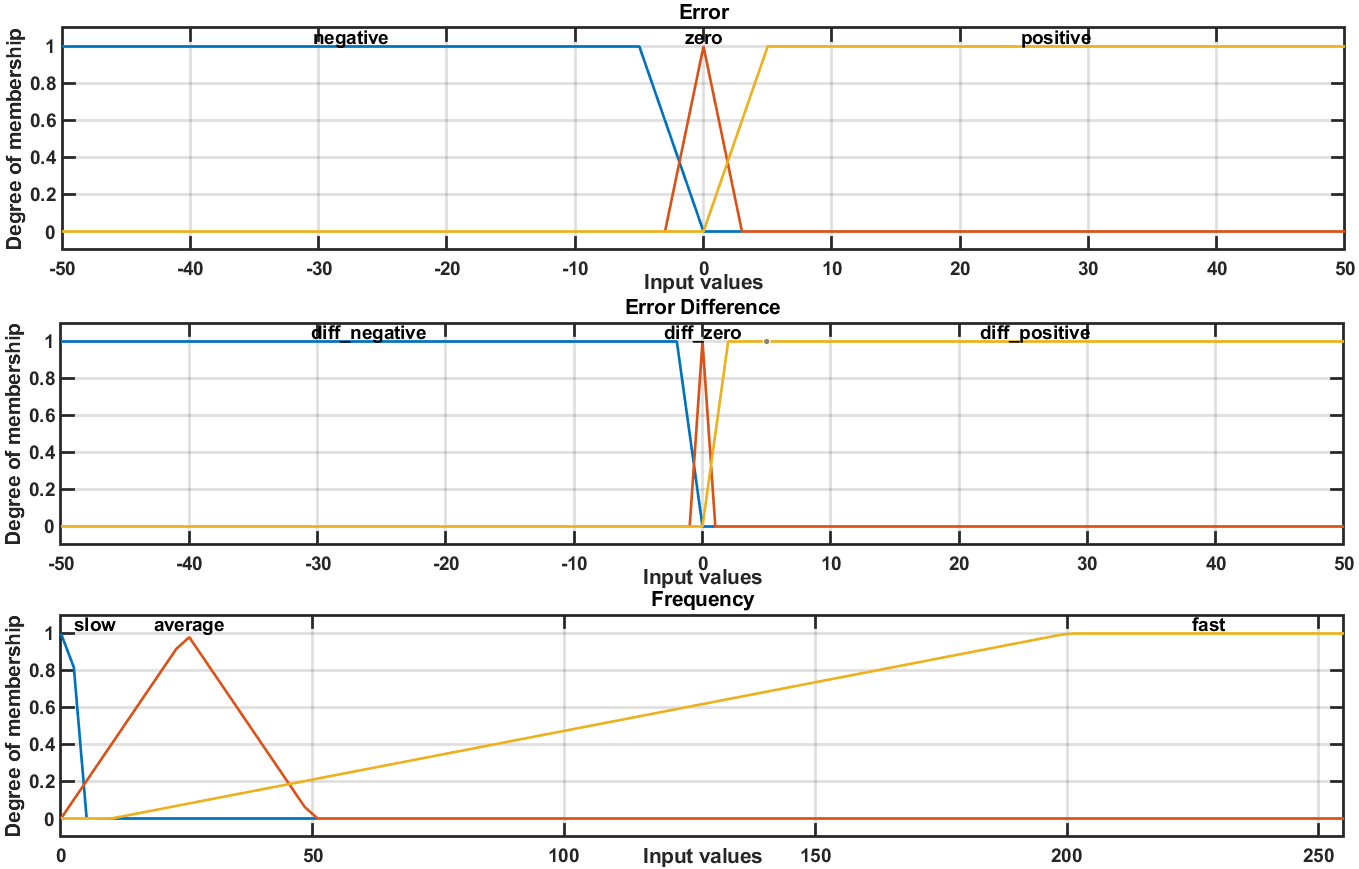
\includegraphics[scale=0.35]{fig2.png}
\caption{Membership functions for the fuzzy system inputs and outputs, designed using the Fuzzy Logic Designer toolbox in MATLAB.}
\label{fig:membership_functions}
\end{figure}

Finally, we defined the \textit{defuzzification process} and the configuration of membership degrees according to the parameters shown in Figure~\ref{fig:defuzzification_config}.  

\begin{figure}[ht]
\centering
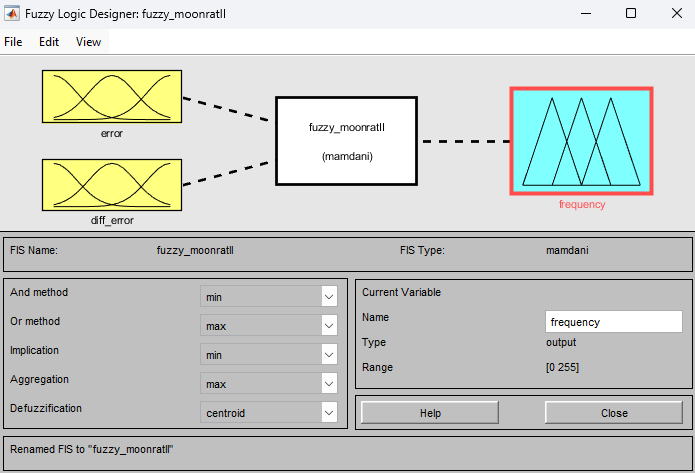
\includegraphics[scale=0.55]{fig3.png}
\caption{Defuzzification and membership function configuration for the fuzzy control system.}
\label{fig:defuzzification_config}
\end{figure}

\printbibliography

\end{document}
